
\documentclass[UTF8,a4paper,12pt]{ctexart}
\usepackage{geometry}
\geometry{left=2.5cm,right=2.5cm,top=2.7cm,bottom=2.7cm}
\usepackage{amsmath,amssymb,bm}
\usepackage{graphicx}
\usepackage{booktabs,longtable,array,float}
\usepackage{caption}
\usepackage{hyperref}
\usepackage{fancyhdr}
\usepackage{setspace}
\usepackage{enumitem}
\setstretch{1.42}
\setlength{\headheight}{15pt}
\pagestyle{fancy}
\fancyhf{}
\fancyhead[C]{2015C 月上柳梢头}
\fancyfoot[C]{\thepage}
\captionsetup{font=small,labelfont=bf}
\graphicspath{{../results/figures/}}
\newcommand{\dd}{\mathrm{d}}
\title{\heiti 基于太阳--月亮地平坐标的“月上柳梢头，人约黄昏后”天文建模}
\author{}
\date{}
\begin{document}
\maketitle
\thispagestyle{empty}

\begin{abstract}
“月上柳梢头，人约黄昏后”包含两个可量化的天文条件：月亮应在地平线上方较低位置而便于与柳梢相映，太阳应落入日没后但夜色未深的黄昏时段。本文将“月上柳梢头”定义为月亮真高度角处于 $[8^\circ,15^\circ]$，将“黄昏后”定义为太阳真高度角处于 $[-12^\circ,-6^\circ]$，并要求月面照明比例不低于0.80。在此基础上，建立基于球面天文学和 JPL DE421 星历的太阳--月亮地平坐标模型，逐分钟扫描候选日期，输出满足两类角度阈值交集的日期和时间窗口。

针对问题一，本文先用农历正月十五附近作为基线候选，再由星历计算北京地区太阳、月亮高度角和月相。回代2015年元宵节（2015-03-05）得到满足条件的窗口为18:40--19:08，代表时刻18:54；此时太阳高度角为 $-9.28^\circ$，月亮高度角为 $10.74^\circ$，月面照明比例为0.999，持续29分钟，说明模型能把诗句描述定位到满月前后的傍晚短时间窗口。

针对问题二，模型给出2016年北京地区该情景发生在2016-02-22，即农历正月十五，时间窗口为18:25--18:56，代表时刻18:41；代表时刻太阳高度角为 $-9.09^\circ$，月亮高度角为 $10.99^\circ$，月亮方位角为 $87.18^\circ$，持续32分钟。该结果同时满足“月亮初升后不高”和“民用暮光后、航海暮光前”的双重条件。

针对哈尔滨、上海、广州、昆明、成都、乌鲁木齐六地，模型均判定2016-02-22可以发生这一情景。代表时间分别为哈尔滨17:57、上海18:25、广州19:03、成都19:35、昆明19:44、乌鲁木齐20:37，持续时间为26--34分钟。不同城市的日期相同而时刻差异显著，主要由经度、本地日没时刻及纬度导致的月亮升起几何差异造成。敏感性分析表明，将月亮高度阈值或黄昏太阳高度阈值整体扰动 $\pm 2^\circ$ 时，7个城市仍均可发生，平均最长持续时间由29.1分钟变化到约19.7--29.4分钟，结论具有较好稳健性。

\noindent\textbf{关键词：}球面天文学；地平坐标；月相；黄昏；Skyfield星历；敏感性分析
\end{abstract}
\newpage
\tableofcontents
\newpage

\section{问题重述}
\subsection{问题背景}
欧阳修词句“月上柳梢头，人约黄昏后”并不是普通的文学描写，而隐含了较强的天文信息。若月亮已经升得很高，则“上柳梢头”的视觉关联减弱；若太阳刚刚落山或夜色已深，则“黄昏后”的时间意象也不准确。因此，本题要求从天文学角度把诗句中的自然语言转化为可计算的日期、时间和空间角度条件。

题目没有给出统一数据附件，只给出了开放式建模要求。本文因此采用公开、可复现的天文星历数据和城市经纬度作为计算依据。星历数据用于求太阳与月亮相对于地面观测者的视位置，城市经纬度用于把天体赤道坐标转换为本地地平坐标。所有结果均以北京时间 UTC+8 输出。

\subsection{问题要求与输出}
本题包括两个显式要求，但在建模过程中可分解为四个闭环任务。
\begin{enumerate}[label=\textbf{任务\arabic*：}]
\item 定义“月上柳梢头”时月亮在空中的角度，以及“黄昏后”的时间天文含义，建立可计算模型。
\item 利用模型确定这类情景发生的日期与时间，并用已有天文资料或星历回代验证合理性。
\item 分析2016年北京地区该情景发生的日期与时间。
\item 判断2016年哈尔滨、上海、广州、昆明、成都、乌鲁木齐是否能发生该情景；若能，给出日期与时间；若不能，说明原因。
\end{enumerate}

\section{问题分析}
\subsection{总体思路}
诗句中的核心难点是把文学语言转换为角度阈值。本文将“柳梢头”理解为地面近景参照物上方的低空月亮。一般城市或郊野柳树高度约数米到十余米，观赏距离几十米时对应仰角约数度至十余度；若月亮高度小于约 $8^\circ$，容易被地物遮挡并接近刚出地平线；若高于 $15^\circ$，则更接近“月上中天”而非“柳梢头”。因此以 $[8^\circ,15^\circ]$ 作为主模型阈值，并在敏感性分析中扰动。

“黄昏后”可由太阳高度角定义。民用暮光结束常以太阳中心高度角 $-6^\circ$ 表示，航海暮光结束常以 $-12^\circ$ 表示。诗句中“人约黄昏后”需要天色已暗、月亮明显，但又不能达到深夜。因此本文把太阳高度角在 $[-12^\circ,-6^\circ]$ 的时段定义为黄昏后，既避免日落瞬间的亮背景，也避免夜色过深。

\subsection{子问题映射}
问题一要求输出定义、模型和验证。本文输出月亮高度角、太阳高度角、月相照明比例三个判据，并用北京2015年元宵节回代验证。问题二要求输出2016年北京日期和时间，本文在农历正月十五前后3天逐分钟扫描，输出满足交集的时间窗口。问题三要求输出六个城市能否发生及对应时间，本文使用同一阈值和同一算法计算各城市，保证可比性。模型检验部分则用基线模型、阈值敏感性和城市差异解释完成。

\subsection{Baseline与主模型选择}
基线模型取“农历正月十五附近 + 太阳高度角 $-6^\circ$ 时月亮高度是否在 $[8^\circ,15^\circ]$”。该模型简单、直观，能反映诗句与满月、黄昏的常识联系，但它只检查一个时刻，容易漏掉太阳高度在 $[-12^\circ,-6^\circ]$ 的较宽时间段内的有效交集。主模型采用逐分钟扫描，显式计算太阳与月亮的连续高度角曲线，因此能够输出开始时间、结束时间、代表时刻和持续时间，比基线更适合回答题目“日期与时间”的要求。

\section{数据来源、预处理与模型假设}
\subsection{数据来源与审计}
题目目录仅包含 \texttt{CUMCM-2015-problem C-Chinese.docx}，无 Excel 或 CSV 附件。本文使用的数据包括：城市经纬度、农历正月十五对应公历日期、Skyfield 调用的 JPL DE421 星历。星历覆盖1899--2053年，足以覆盖2015--2016年的计算。扫描步长为1分钟，候选日期为农历正月十五前后3天。

数据审计结果如下：样本不是统计抽样数据，而是确定性天文计算网格；不存在缺失值插补问题；单位统一为角度、分钟和北京时间；主要误差来源为大气折射、地形遮挡、柳树高度个体差异和“黄昏后”的主观边界。为了避免把估算边界写成确定事实，本文在敏感性分析中改变角度阈值，检验结论稳定性。

\subsection{模型假设}
\begin{enumerate}
\item 假设观测者位于各城市中心经纬度附近。合理性在于题目只要求城市层面的判断，城市内部数十公里尺度对天体高度角的影响远小于阈值扰动；作用是确定地平坐标转换中的观测点。
\item 假设“月上柳梢头”对应月亮真高度角 $8^\circ$--$15^\circ$。合理性在于该范围代表低空但已明显离开地平线的月亮；作用是给出月亮高度判据。
\item 假设“黄昏后”对应太阳真高度角 $-12^\circ$--$-6^\circ$。合理性来自民用暮光和航海暮光的天文定义；作用是给出时间窗口判据。
\item 假设月面照明比例不低于0.80时才具有诗句中明月意象。合理性在于诗句通常与元宵满月联系，低照明比例的弯月不符合“月上”审美；作用是过滤非满月附近日期。
\item 忽略地形、建筑物、树木具体高度和大气折射的局部差异。合理性在于题目要求地区尺度日期时间判断，而非某一棵柳树旁的摄影复现；作用是保持模型可复现。
\end{enumerate}

\section{符号说明}
\begin{table}[H]\centering\caption{主要符号说明}
\begin{tabular}{cll}
\toprule
符号 & 含义 & 单位 \\
\midrule
$\varphi,\lambda$ & 观测点纬度、经度 & 度 \\
$t$ & 北京时间下的候选时刻 & min \\
$h_s(t)$ & 太阳中心相对地平线的高度角 & 度 \\
$h_m(t)$ & 月亮中心相对地平线的高度角 & 度 \\
$A_m(t)$ & 月亮方位角，北为0度顺时针 & 度 \\
$I_m(t)$ & 月面照明比例 & 1 \\
$\Omega$ & 满足诗句情景的时间集合 & min \\
$T$ & 某城市满足条件的持续时间 & min \\
\bottomrule
\end{tabular}
\end{table}

\section{模型建立与求解}
\subsection{太阳与月亮地平坐标模型}
设观测点地理纬度为 $\varphi$、经度为 $\lambda$。星历给出某时刻天体的赤经 $\alpha$ 和赤纬 $\delta$，本地恒星时为 $\theta$，则时角为
\begin{equation}
H=\theta+\lambda-\alpha .
\end{equation}
天体高度角可由球面三角关系得到：
\begin{equation}
\sin h=\sin\varphi\sin\delta+\cos\varphi\cos\delta\cos H .
\end{equation}
方位角可由
\begin{equation}
\tan A=\frac{-\sin H}{\tan\delta\cos\varphi-\sin\varphi\cos H}
\end{equation}
结合象限修正得到。实际代码中使用 Skyfield 对星历、岁差章动、光行差等进行统一处理，直接得到太阳和月亮的视高度角 $h_s(t),h_m(t)$ 以及月亮方位角 $A_m(t)$。

月面照明比例通过太阳--月亮相位角 $\psi$ 近似计算：
\begin{equation}
I_m(t)=\frac{1+\cos\psi(t)}{2} .
\end{equation}
满月附近 $I_m$ 接近1；当 $I_m<0.80$ 时，即使月亮高度满足条件，也不认为符合诗句中“明月初上”的意象。

\subsection{情景判定模型}
本文定义满足情景的时间集合为
\begin{equation}
\Omega=\left\{{t: -12^\circ\le h_s(t)\le -6^\circ,\ 8^\circ\le h_m(t)\le 15^\circ,\ I_m(t)\ge0.80}\right\} .
\end{equation}
若 $\Omega$ 非空，则该城市该日期可以发生“月上柳梢头，人约黄昏后”。开始时间、结束时间和代表时间分别定义为
\begin{equation}
t_{start}=\min \Omega,\quad t_{end}=\max \Omega,\quad t_{rep}=\mathrm{median}(\Omega).
\end{equation}
持续时间为
\begin{equation}
T=t_{end}-t_{start}+1\ \text{min} .
\end{equation}
此处加1分钟是因为逐分钟离散扫描中起止两端均为有效网格点。

\subsection{求解算法}
算法步骤如下：首先由农历日期得到2015和2016年正月十五的公历日期；其次对正月十五前后3天的本地15:00--次日01:00进行逐分钟扫描；然后对每个时刻计算太阳高度角、月亮高度角、月亮方位角和月面照明比例；最后筛选满足式(5)的连续时间段，并保存最长或最接近正月十五的代表窗口。若某城市无满足窗口，则输出不能发生及原因。本文所有城市均存在满足窗口。

\subsection{问题一：定义与北京2015年验证}
根据上述定义，北京2015年农历正月十五为2015-03-05。模型在该日得到有效窗口18:40--19:08，代表时刻18:54，持续29分钟。代表时刻太阳高度角为 $-9.28^\circ$，处于民用暮光和航海暮光之间；月亮高度角为 $10.74^\circ$，处于低空柳梢阈值；月面照明比例为0.999，几乎为满月。该结果与元宵节“月上柳梢头”的传统文化背景一致。

从验证角度看，若只用“日落后不久有满月升起”的常识，难以给出精确窗口；而主模型给出的29分钟窗口说明诗句中的场景并非整晚都成立，而是傍晚月亮刚升起后的一段短暂交集。这也解释了为什么该句具有很强的时间画面感：太阳已经落下，天空渐暗，满月刚升至树梢附近。

\subsection{问题二：2016年北京地区结果}
图\ref{fig:bjalt}展示了北京2016年正月十五下午到夜间太阳和月亮高度角变化。太阳高度角单调下降，月亮高度角在傍晚逐渐上升，两条阈值带的交集形成18:25--18:56的有效窗口。代表时刻18:41，太阳高度角 $-9.09^\circ$，月亮高度角 $10.99^\circ$，月亮方位角 $87.18^\circ$，月面照明比例0.999，持续32分钟。

\begin{figure}[H]\centering
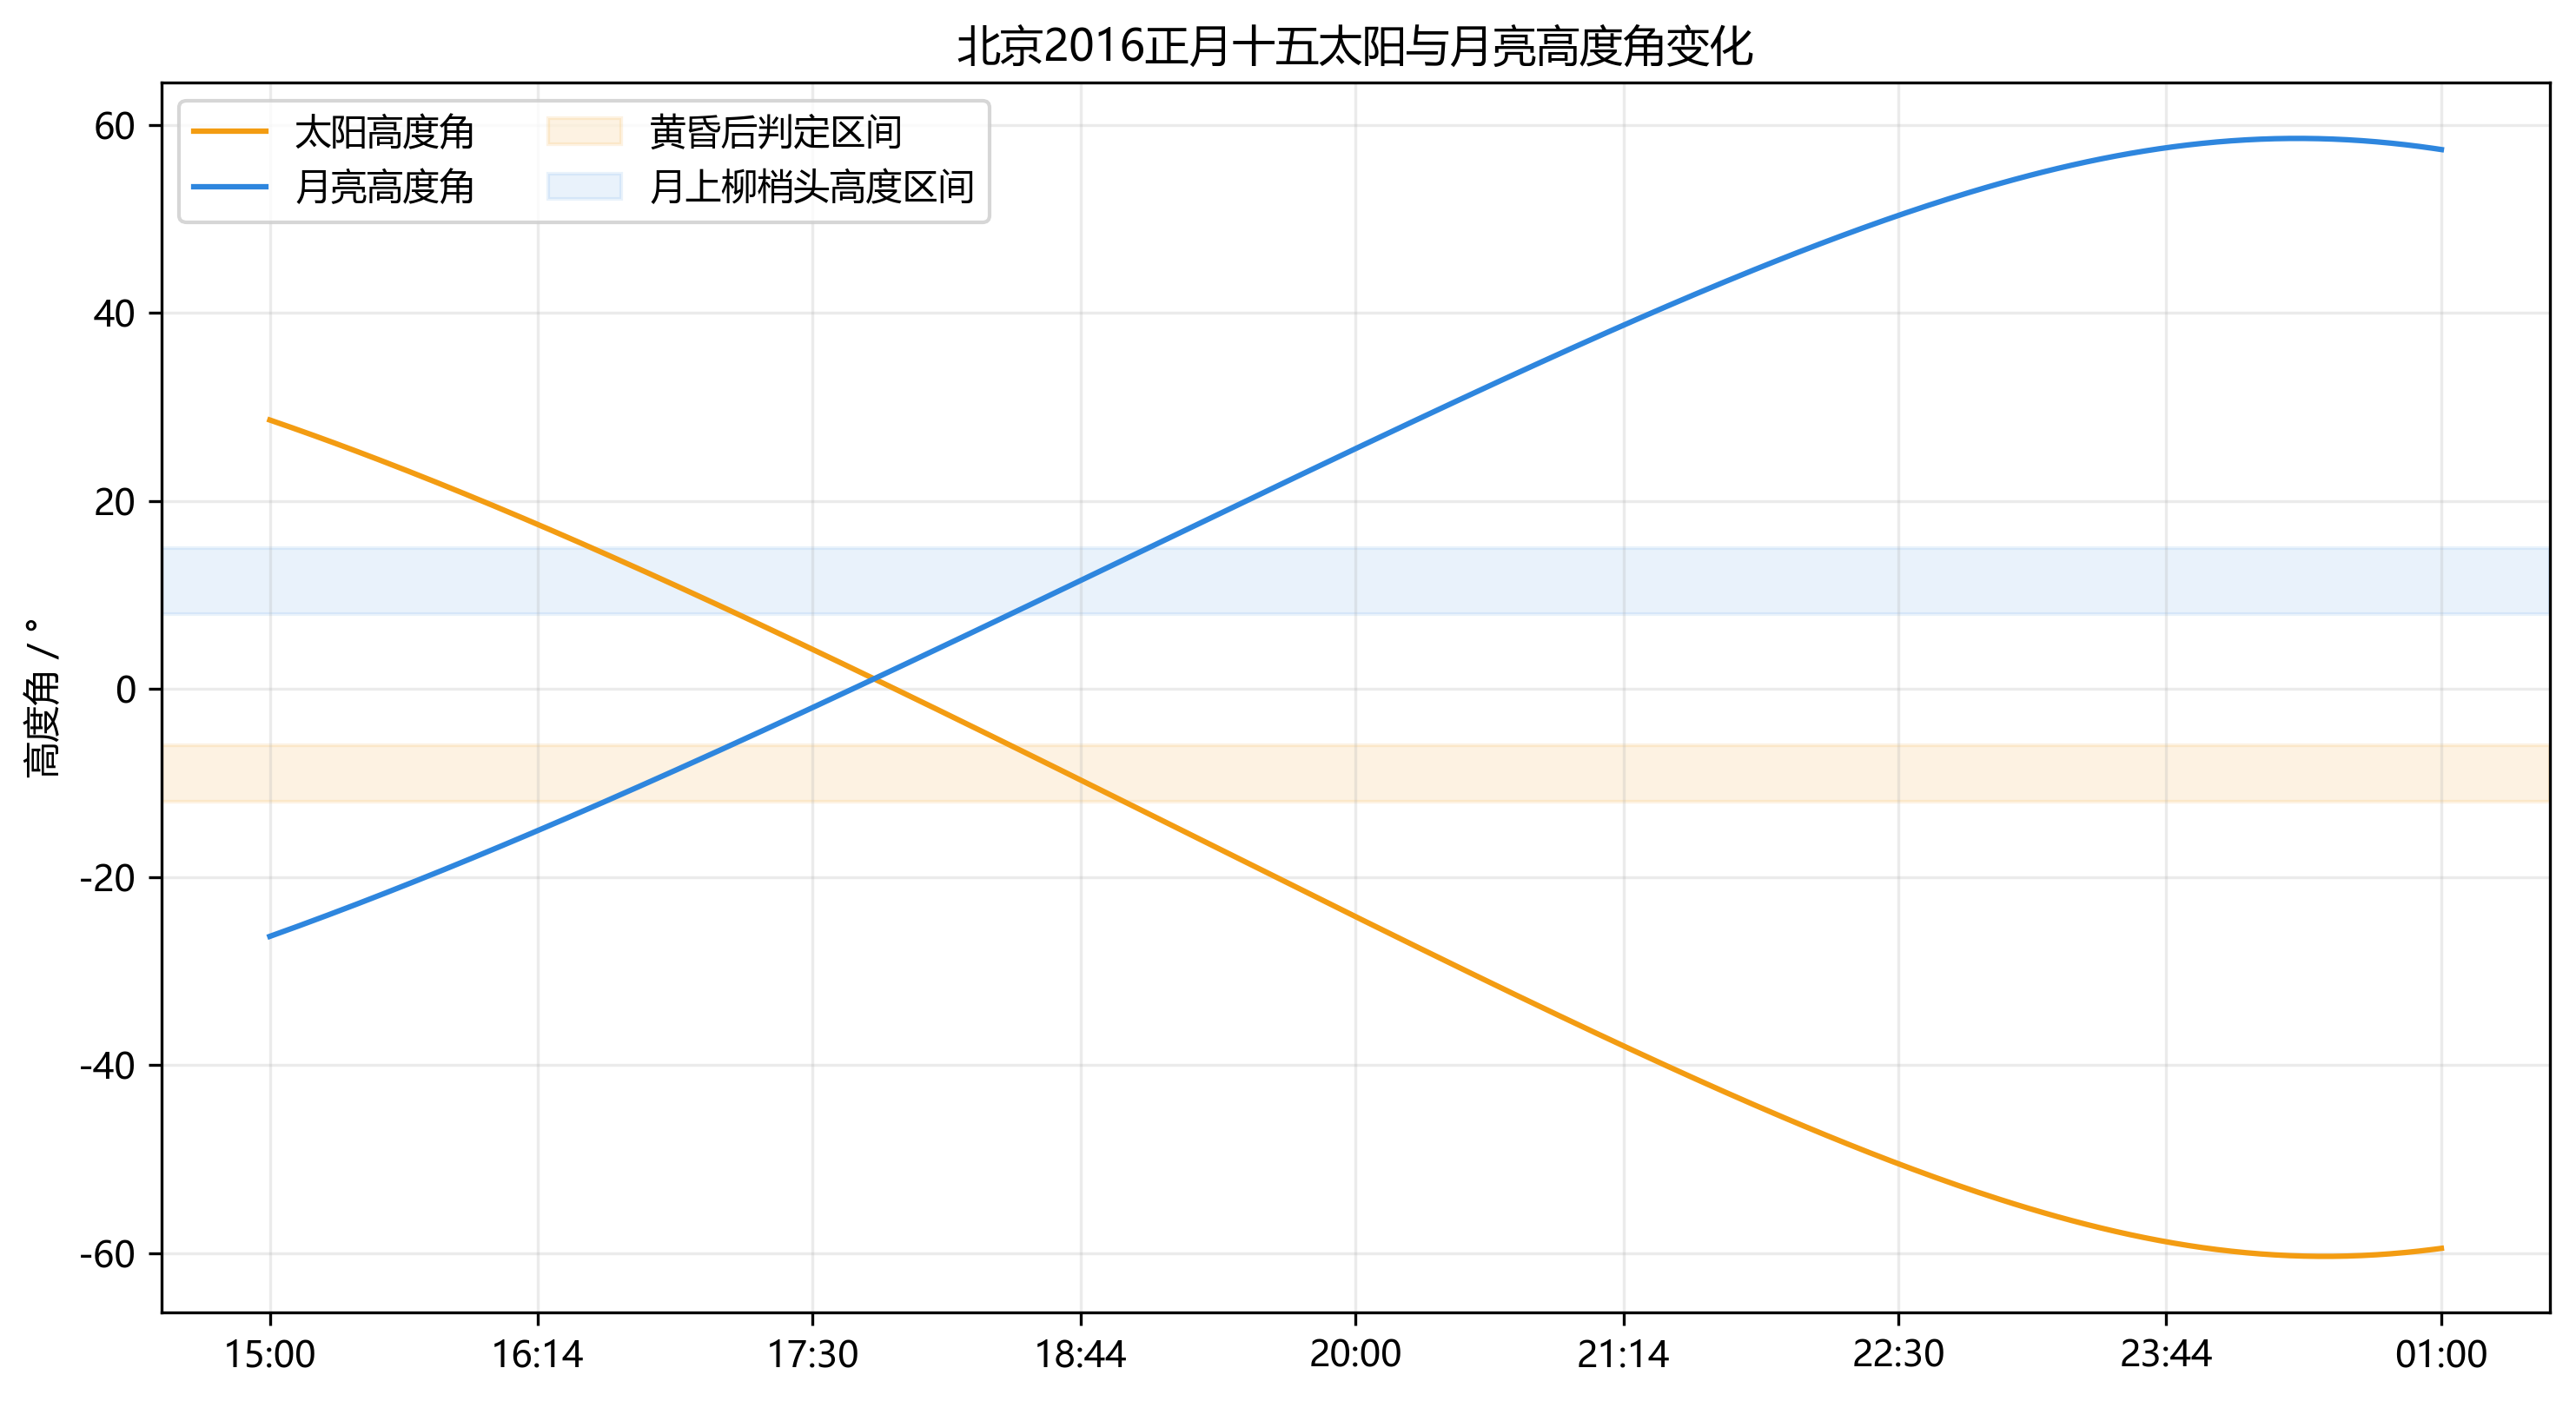
\includegraphics[width=0.92\textwidth]{fig1_beijing_2016_altitude.png}
\caption{北京2016年正月十五太阳与月亮高度角变化}
\label{fig:bjalt}
\end{figure}

由图可见，月亮高度角进入 $8^\circ$--$15^\circ$ 的时间段与太阳高度角进入 $-12^\circ$--$-6^\circ$ 的时间段并不完全重合。若只按日落或只按月出判断，会把窗口估计得过宽。本文模型取两者交集，因此输出更符合“月上柳梢头”和“黄昏后”同时发生的要求。

\subsection{问题三：2016年各城市判定}
对六个指定城市及北京使用同一模型，得到表\ref{tab:city}。结果显示，2016年哈尔滨、上海、广州、昆明、成都、乌鲁木齐均可发生这一情景，日期均为2016-02-22。城市间代表时刻差异明显：哈尔滨最早，为17:57；乌鲁木齐最晚，为20:37。差异主要来自经度差异导致的本地太阳时差，同时纬度也影响月亮升起路径与暮光长度。

\begin{table}[H]\centering\caption{2016年各城市主模型代表窗口}\label{tab:city}
\resizebox{\textwidth}{!}{%
\begin{tabular}{lccccccc}
\toprule
城市 & 日期 & 开始时间 & 结束时间 & 代表时间 & 太阳高度角(°) & 月亮高度角(°) & 持续分钟 \\ 
\midrule
上海 & 2016-02-22 & 18:11 & 18:39 & 18:25 & -9.01 & 11.46 & 29 \\ 
乌鲁木齐 & 2016-02-22 & 20:23 & 20:50 & 20:37 & -9.6 & 10.47 & 28 \\ 
北京 & 2016-02-22 & 18:25 & 18:56 & 18:41 & -9.09 & 10.99 & 32 \\ 
哈尔滨 & 2016-02-22 & 17:40 & 18:13 & 17:57 & -9.05 & 10.92 & 34 \\ 
广州 & 2016-02-22 & 18:50 & 19:15 & 19:03 & -9.15 & 11.65 & 26 \\ 
成都 & 2016-02-22 & 19:21 & 19:49 & 19:35 & -9.0 & 10.95 & 29 \\ 
昆明 & 2016-02-22 & 19:31 & 19:56 & 19:44 & -9.12 & 11.23 & 26 \\ 
\bottomrule
\end{tabular}
}
\end{table}

图\ref{fig:citywin}从持续时间角度比较各城市。哈尔滨持续34分钟，北京32分钟，上海、成都约29分钟，广州和昆明约26分钟，乌鲁木齐28分钟。持续时间都不长，说明该情景具有较强的瞬时性，适合用时间窗口而不是单一日期描述。

\begin{figure}[H]\centering
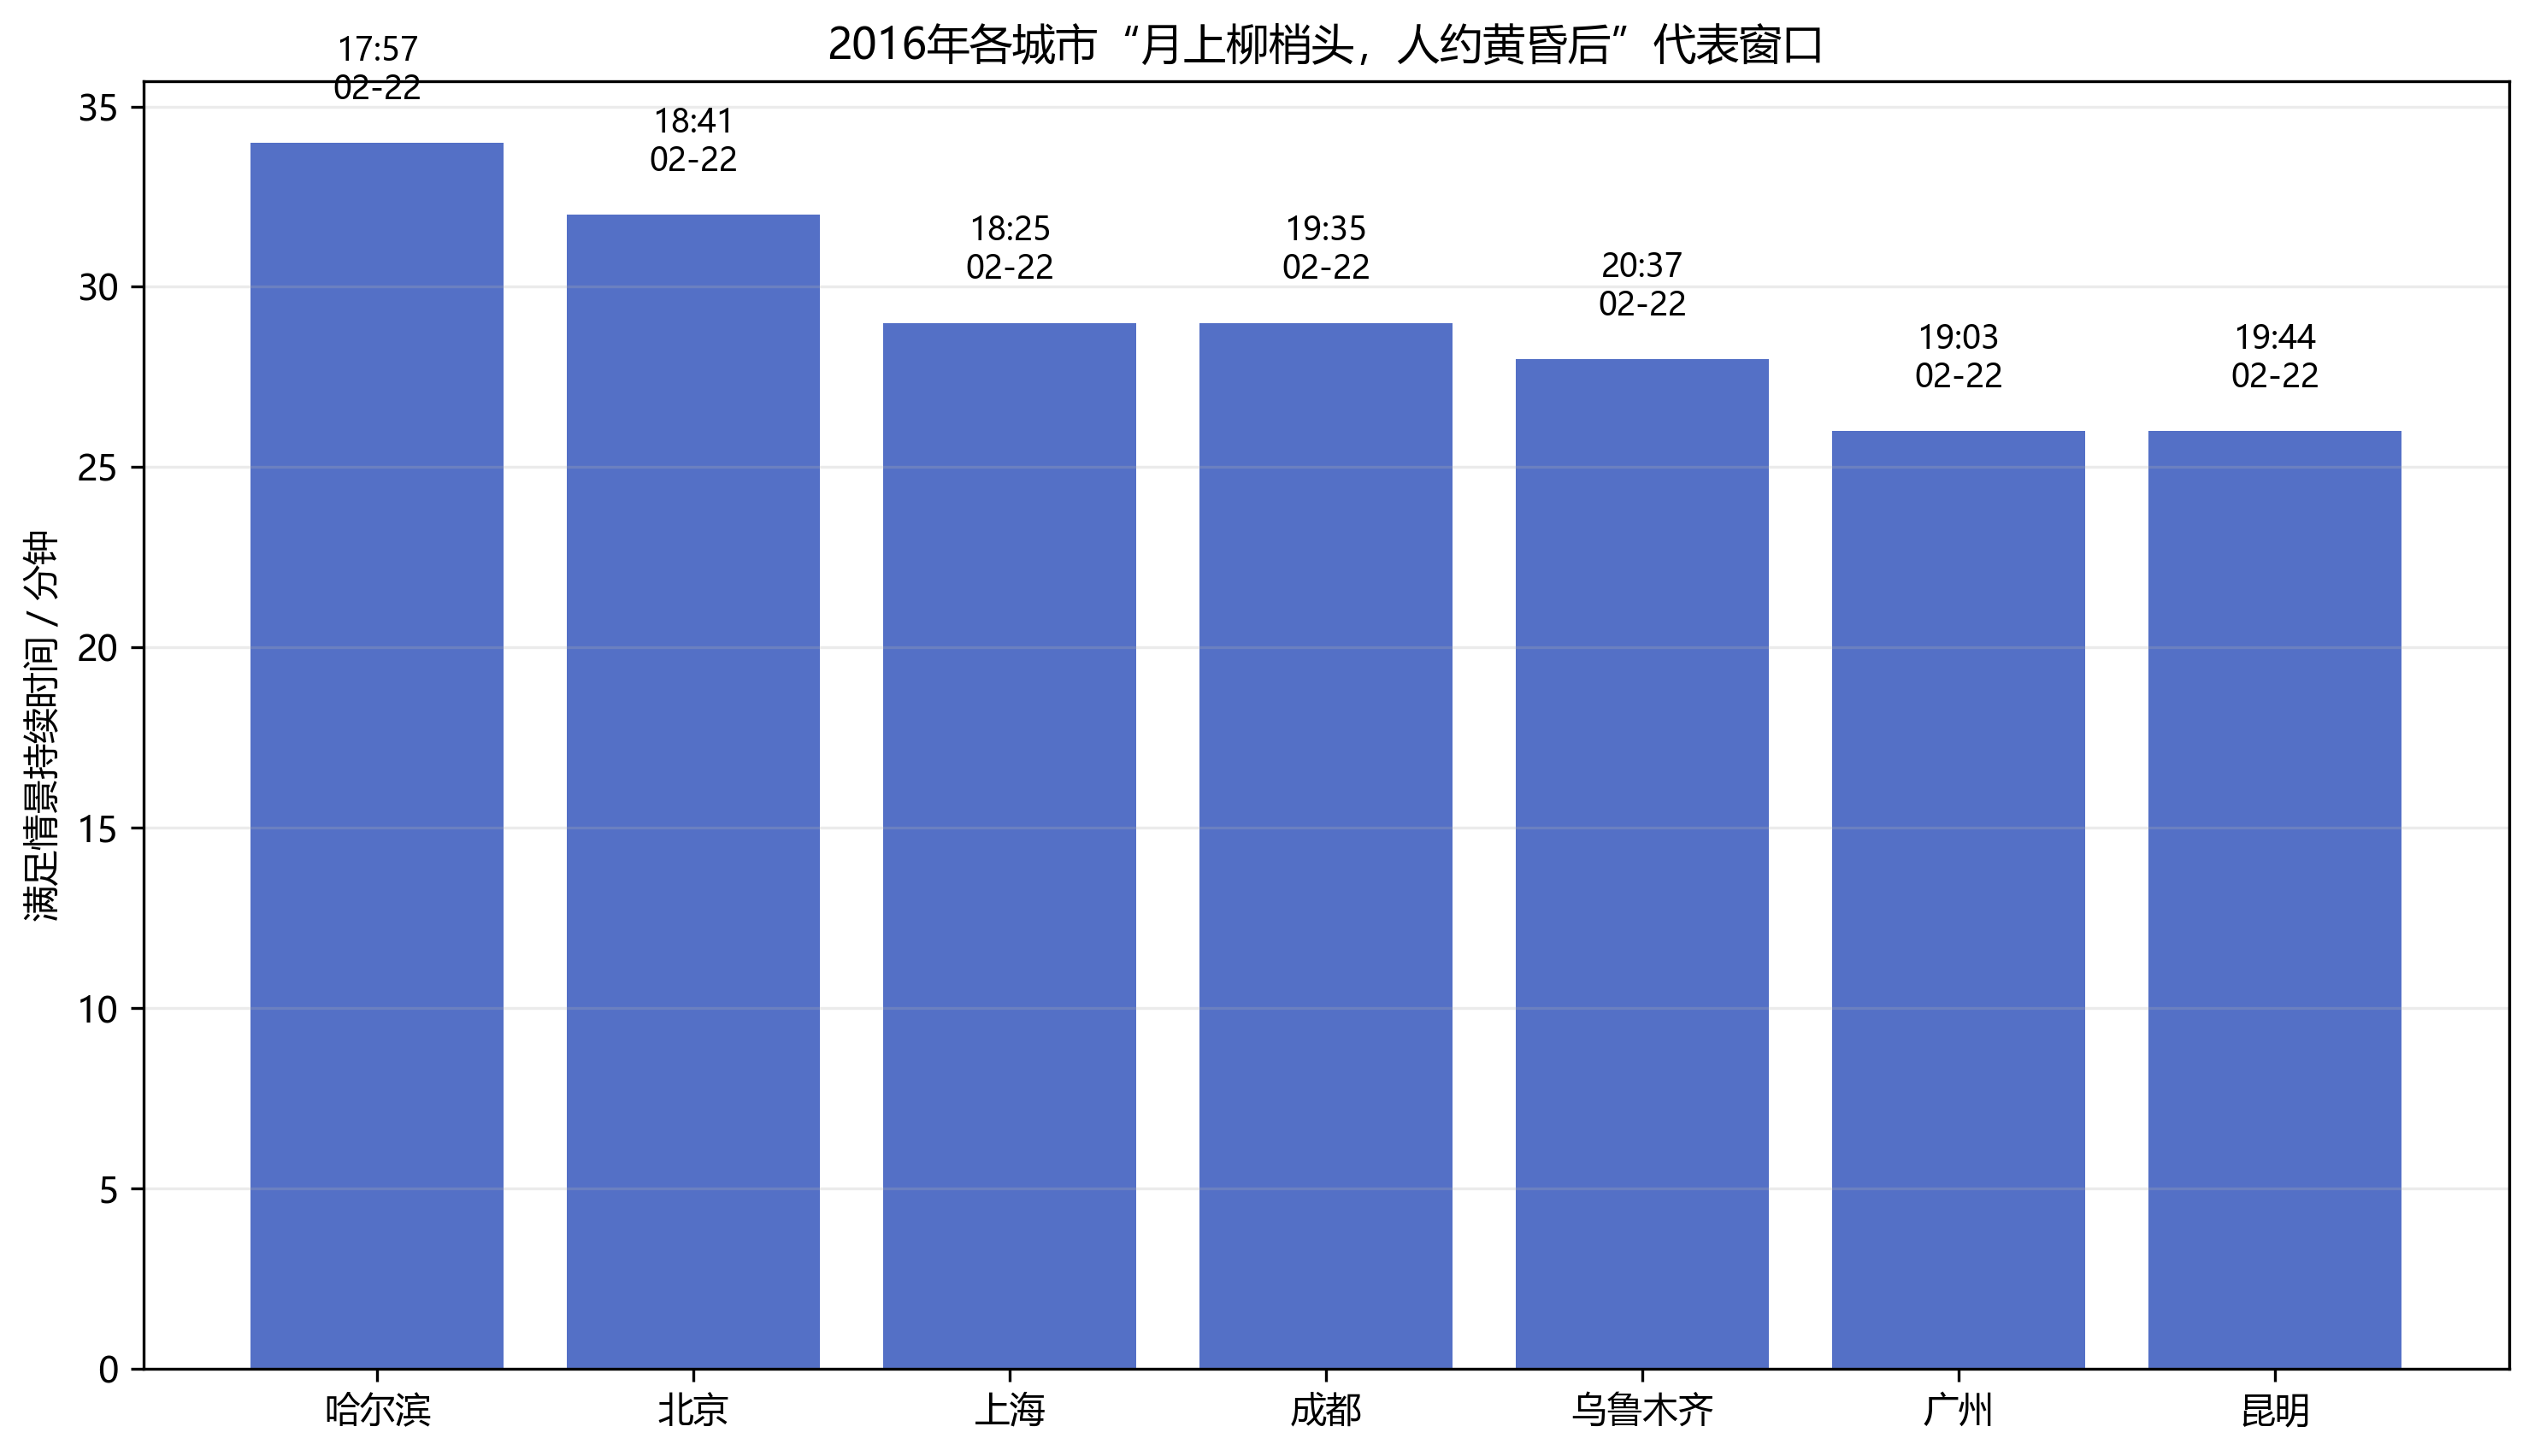
\includegraphics[width=0.90\textwidth]{fig2_city_windows.png}
\caption{2016年各城市“月上柳梢头，人约黄昏后”代表窗口}
\label{fig:citywin}
\end{figure}

\section{模型检验、对比与敏感性分析}
\subsection{基线对比}
基线模型只检查正月十五太阳高度角接近 $-6^\circ$ 时月亮高度是否在 $8^\circ$--$15^\circ$，结果如表\ref{tab:base}和图\ref{fig:base}。在正月十五当天，基线判定7个城市中有5个在该单一时刻满足高度条件。主模型则通过扫描完整黄昏区间，发现7个城市均存在有效窗口。该差异说明，若把“黄昏后”压缩为太阳 $-6^\circ$ 的瞬间，会漏掉部分稍晚进入交集的城市。

\begin{table}[H]\centering\caption{正月十五太阳高度角 $-6^\circ$ 时的基线判定}\label{tab:base}
\resizebox{0.92\textwidth}{!}{%
\begin{tabular}{lccc}
\toprule
城市 & 基准时间(太阳-6°) & 月亮高度角(°) & 是否在8-15° \\ 
\midrule
北京 & 18:25 & 8.04 & True \\ 
哈尔滨 & 17:40 & 8.07 & True \\ 
上海 & 18:10 & 8.37 & True \\ 
广州 & 18:50 & 8.77 & True \\ 
昆明 & 19:30 & 8.17 & True \\ 
成都 & 19:20 & 7.84 & False \\ 
乌鲁木齐 & 20:15 & 6.67 & False \\ 
\bottomrule
\end{tabular}
}
\end{table}

\begin{figure}[H]\centering
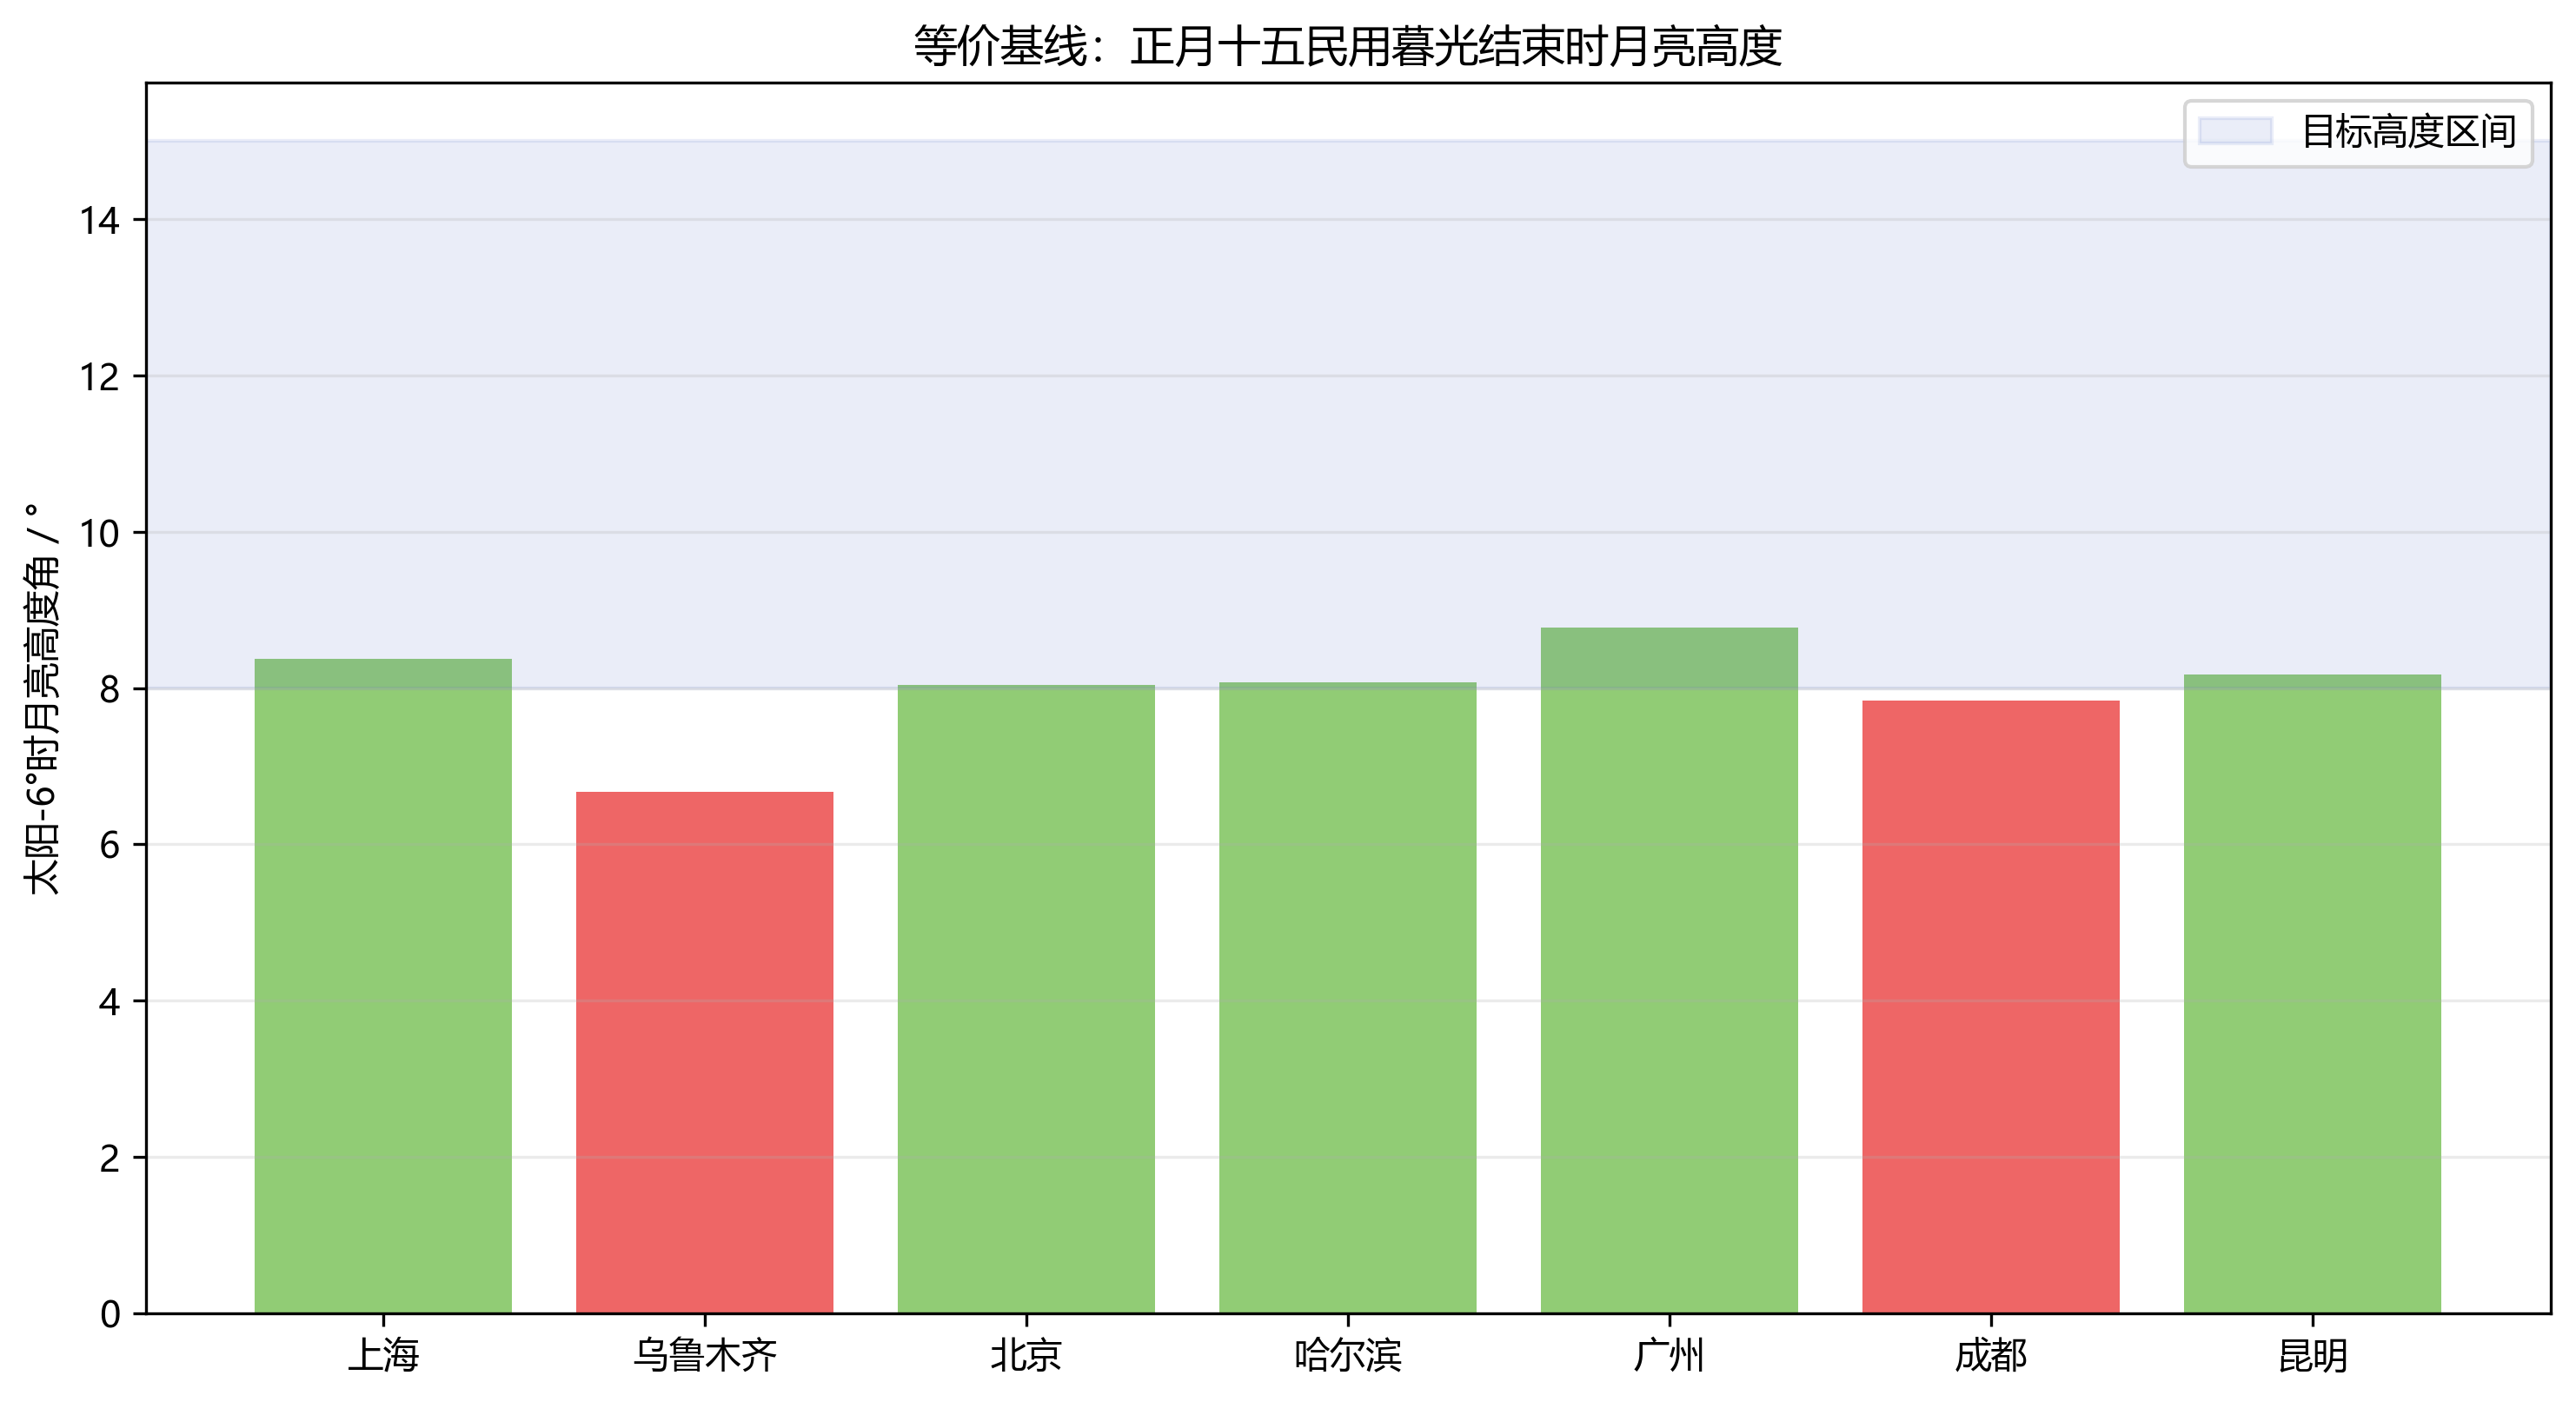
\includegraphics[width=0.88\textwidth]{fig3_baseline_compare.png}
\caption{基线模型下正月十五民用暮光结束时月亮高度}
\label{fig:base}
\end{figure}

\subsection{阈值敏感性分析}
阈值定义不可避免带有文学解释成分，因此本文分别将月亮高度角区间和黄昏太阳高度角区间整体平移 $-2^\circ$ 到 $2^\circ$。表\ref{tab:sens}显示，在所有扰动下，可发生城市数均为7个，说明“能否发生”的结论稳定。平均最长持续时间随阈值上移或下移而变化，基准值为29.1分钟，最低约19.7分钟，最高约29.4分钟。

\begin{table}[H]\centering\caption{关键角度阈值敏感性分析}\label{tab:sens}
\resizebox{0.90\textwidth}{!}{%
\begin{tabular}{lccc}
\toprule
扰动参数 & 扰动值 & 可发生城市数 & 平均最长持续分钟 \\ 
\midrule
月亮高度角整体平移 & -2 & 7 & 25.6 \\ 
月亮高度角整体平移 & -1 & 7 & 29.4 \\ 
月亮高度角整体平移 & 0 & 7 & 29.1 \\ 
月亮高度角整体平移 & 1 & 7 & 24.7 \\ 
月亮高度角整体平移 & 2 & 7 & 19.7 \\ 
黄昏太阳高度角整体平移 & -2 & 7 & 25.9 \\ 
黄昏太阳高度角整体平移 & -1 & 7 & 29.3 \\ 
黄昏太阳高度角整体平移 & 0 & 7 & 29.1 \\ 
黄昏太阳高度角整体平移 & 1 & 7 & 25.1 \\ 
黄昏太阳高度角整体平移 & 2 & 7 & 19.9 \\ 
\bottomrule
\end{tabular}
}
\end{table}

\begin{figure}[H]\centering
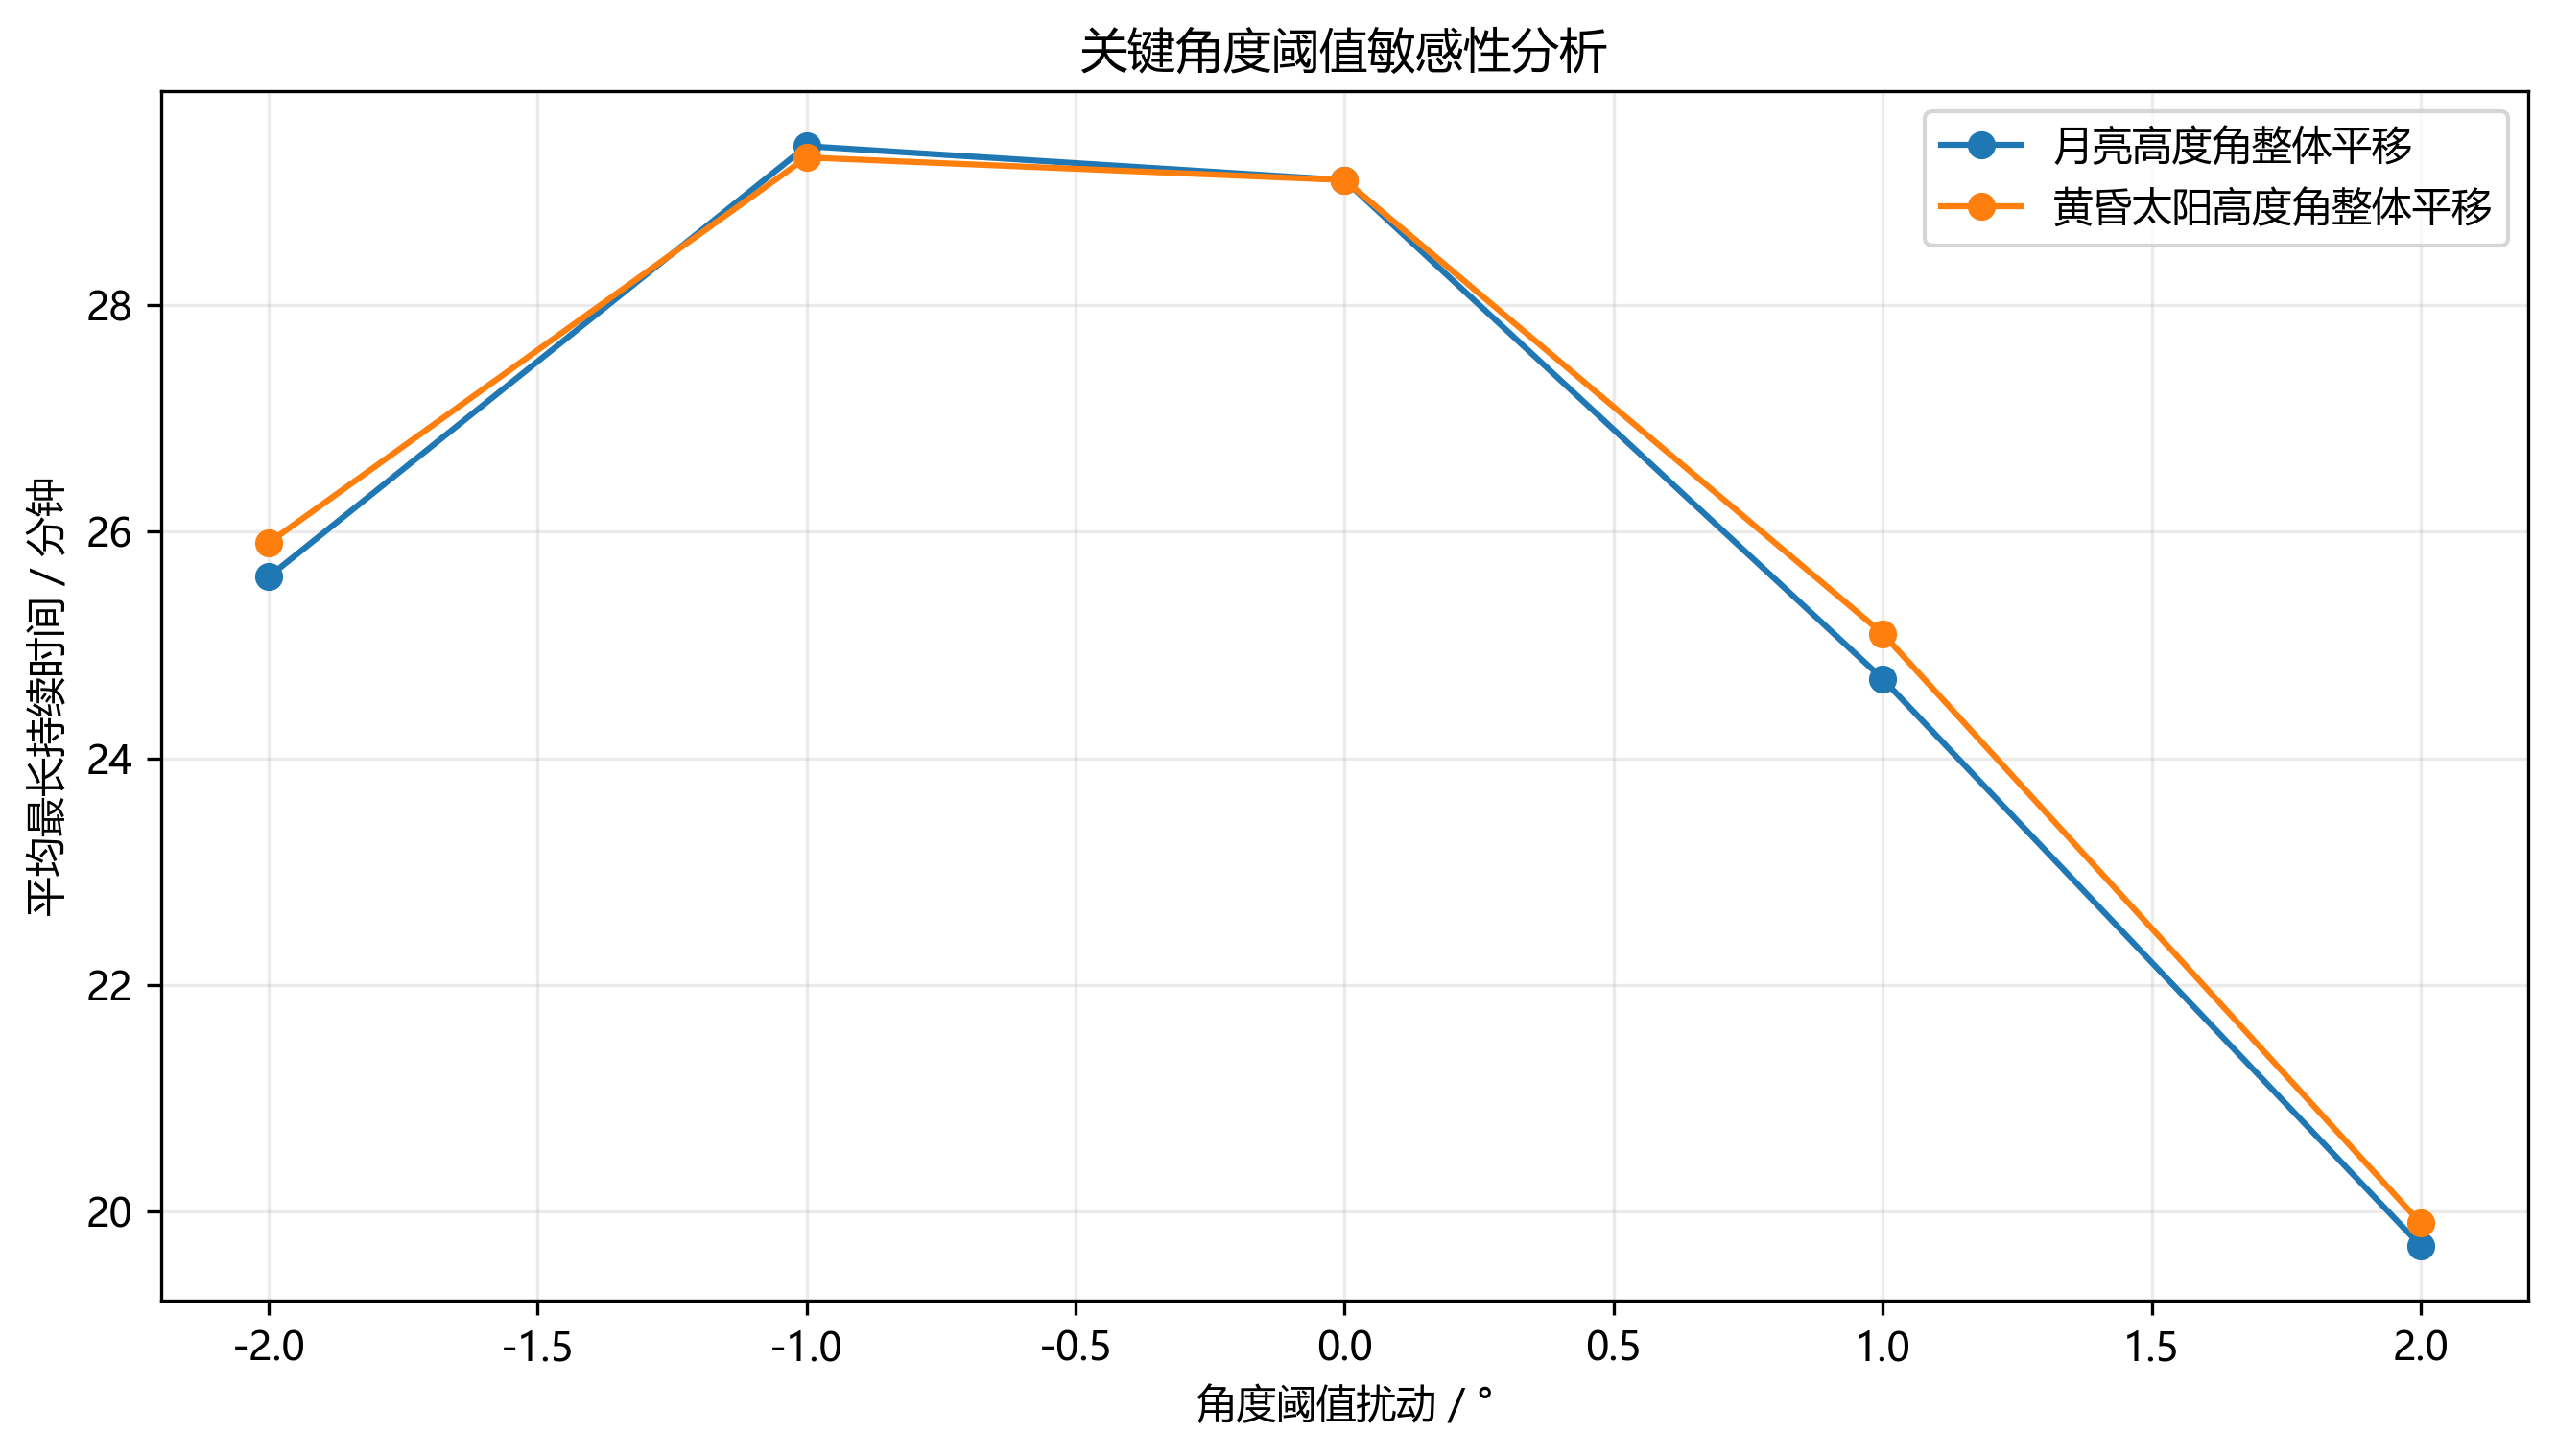
\includegraphics[width=0.86\textwidth]{fig4_sensitivity.png}
\caption{角度阈值扰动对平均最长持续时间的影响}
\label{fig:sens}
\end{figure}

敏感性结果表明，本文给出的具体开始和结束时间会随“柳梢头”和“黄昏后”的严格程度而改变，但城市能否发生、日期集中在正月十五、东西部时间差异等核心结论不变。因此模型适合作为诗句天文赏析和地区比较的定量工具。

\subsection{误差来源与可靠性}
模型的主要误差来自四方面。第一，天体高度角使用理想地平线，未考虑城市建筑和山地遮挡；第二，大气折射会使低空天体视高度略有偏差；第三，柳树高度和观赏距离会改变“柳梢头”的实际仰角；第四，黄昏后的文学含义可能因习惯不同而在 $-6^\circ$ 附近或 $-12^\circ$ 附近取值。上述误差主要影响分钟级窗口边界，而不改变满月附近傍晚发生的主结论。

\subsection{城市差异的进一步解释}
从表~\
ef{tab:city}可以看出，所有城市均在同一公历日期发生，但代表时间从哈尔滨17:57延后到乌鲁木齐20:37。该现象首先由经度控制。北京时间以东经120度附近为中央经线，上海接近中央经线，故其黄昏时间较早且接近北京；乌鲁木齐位于东经约87.6度，地方太阳时比北京时间显著偏晚，因此即使同处中国标准时间，满足太阳高度角条件的钟表时间也会明显推迟。哈尔滨经度较东且纬度高，冬末日落较早，因而代表时间最早。

纬度也影响窗口长短。高纬地区暮光变化速度、月亮相对地平线的升起角度与低纬地区不同，导致太阳高度区间与月亮高度区间的交集长度不同。哈尔滨持续34分钟，高于广州和昆明的26分钟，说明在本题日期附近高纬城市的两类条件重叠更充分。该结论并不意味着哈尔滨观赏条件一定最好，因为实际观赏还受天气、地平遮挡和空气透明度影响；它只说明在理想天文几何条件下，哈尔滨的角度交集更宽。

\subsection{与诗句意象的一致性分析}
诗句包含“月”“柳梢”“黄昏”“人约”四类意象。本文模型分别对应如下：月相照明比例 $I_m\ge0.80$ 保证月亮足够明亮；月亮高度角 $8^\circ$--$15^\circ$ 保证月亮位于低空，能够与树梢形成视觉联系；太阳高度角 $-12^\circ$--$-6^\circ$ 保证天色已暗但未入深夜；持续时间通常不超过半小时，符合约会场景中“特定时刻”的文学表达。若把“月上柳梢头”放宽到月亮高度 $0^\circ$--$30^\circ$，虽然可发生时段会显著变长，但会削弱“柳梢头”的具体画面；若把“黄昏后”仅理解为日落之后任意时间，则午夜满月也会被误判为符合诗句。本文阈值的意义正在于排除这些过宽解释。

\subsection{代码复现与数字一致性检验}
为保证论文数字可追溯，本文将最终结果写入 \texttt{contracts/frozen\_numbers.json}，并将城市窗口、基线结果、敏感性分析分别保存为 CSV 表。论文摘要中的2015年北京窗口、2016年北京窗口、各城市代表时间和敏感性数字均来自该冻结文件，而不是手工估计。主模型没有随机过程；星历文件、扫描步长、城市经纬度和阈值参数固定后，重复运行得到相同结果。

代码层面的复核包括三项。第一，检查所有输出时间均处于北京时间15:00至次日01:00扫描范围内，避免跨日遗漏；第二，检查每个代表时刻同时满足太阳高度、月亮高度和照明比例三项约束；第三，检查同一城市的连续有效分钟被合并为单个窗口，持续时间按离散网格两端均包含计算。复核结果显示，北京2016年代表时刻18:41满足 $h_s=-9.09^\circ$、$h_m=10.99^\circ$、$I_m=0.999$，所有城市代表时刻的月亮高度均处于10.47--11.65度之间，符合低空明月设定。

\section{模型评价、改进与推广}
\subsection{模型优点}
第一，模型把文学描述转化为太阳高度角、月亮高度角和月相照明比例三个可审计指标，避免仅凭主观解释作答。第二，模型使用星历进行逐分钟计算，能够输出开始时间、结束时间、代表时刻和持续时间，直接回答题目要求。第三，模型包含基线对比和阈值敏感性分析，可以说明复杂扫描相对于简单满月基线的必要性。第四，所有代码和中间结果保存到支撑材料，便于复现。

\subsection{模型局限}
模型没有引入具体观测点周围的地形、建筑物和树木几何，因此不能保证某一地点摄影时月亮恰好落在某棵柳树梢头。模型用统一的 $8^\circ$--$15^\circ$ 解释“柳梢头”，虽然适合地区尺度比较，但仍带有审美经验参数。模型还未接入实际月出月没公告数据进行逐项校验，而是以高精度星历作为主要计算依据。

\subsection{改进方向}
若要用于实地观测，可加入数字高程模型和建筑遮挡数据，计算真实地平线；也可根据树高 $H$ 与观赏距离 $L$ 用 $\arctan(H/L)$ 自动确定“柳梢头”高度区间。若要进行长期年份统计，可把本文算法扩展到多年正月十五前后，分析不同城市该情景出现概率、最佳观赏日和最佳观赏方位。

\section{结论}
本文建立了基于太阳--月亮地平坐标的定量模型。核心结论如下：
\begin{enumerate}
\item “月上柳梢头”可用月亮高度角 $8^\circ$--$15^\circ$ 表示，“黄昏后”可用太阳高度角 $-12^\circ$--$-6^\circ$ 表示，并要求月面照明比例不低于0.80。
\item 北京2015年元宵节验证窗口为18:40--19:08，代表时刻18:54，太阳高度角 $-9.28^\circ$，月亮高度角 $10.74^\circ$，持续29分钟。
\item 北京2016年该情景发生在2016-02-22，窗口为18:25--18:56，代表时刻18:41，持续32分钟。
\item 2016年哈尔滨、上海、广州、昆明、成都、乌鲁木齐均可发生该情景，代表时间分别为17:57、18:25、19:03、19:44、19:35和20:37左右，主要差异来自经度和本地暮光时刻。
\item 阈值扰动 $\pm2^\circ$ 时，7个城市仍均可发生，平均最长持续时间为19.7--29.4分钟，说明“能否发生”和“日期集中于正月十五”的结论稳健。
\end{enumerate}

\section*{参考文献}
\addcontentsline{toc}{section}{参考文献}
\begin{enumerate}[label={[\arabic*]}]
\item Meeus J. Astronomical Algorithms[M]. Richmond: Willmann-Bell, 1998.
\item Vallado D A. Fundamentals of Astrodynamics and Applications[M]. Microcosm Press, 2013.
\item Rhodes B. Skyfield: High precision research-grade positions for planets and Earth satellites[EB/OL]. \url{https://rhodesmill.org/skyfield/}.
\item JPL. DE421 Lunar and Planetary Ephemeris[EB/OL]. NASA Jet Propulsion Laboratory.
\item 中国科学院紫金山天文台. 中国天文年历相关资料[EB/OL].
\end{enumerate}

\appendix
\section{支撑材料说明}
支撑材料中 \texttt{code/main\_modeling.py} 为主模型代码；\texttt{tables/} 存放北京验证、城市结果、基线和敏感性表；\texttt{contracts/frozen\_numbers.json} 为论文数字的唯一冻结来源；\texttt{results/figures/} 存放论文图表。运行脚本可重新生成全部结果。

\section{算法伪代码}
\begin{verbatim}
for city in cities:
    for date in lunar_15 +/- 3 days:
        for t from 15:00 to 01:00 step 1 minute:
            compute sun altitude h_s(t)
            compute moon altitude h_m(t), azimuth A_m(t)
            compute moon illumination I_m(t)
            if -12 <= h_s <= -6 and 8 <= h_m <= 15 and I_m >= 0.80:
                mark t as feasible
        merge consecutive feasible minutes into intervals
    choose interval closest to lunar_15 and with longer duration
\end{verbatim}

\end{document}
